
\section*{ Android Studio}
\label{\detokenize{dev_docs:android-studio}}
Android Studio es el entorno de desarrollo integrado (IDE por sus siglas en
inglés) oficial para desarrollar sobre la plataforma Android, está basado en
el popular IntelliJ IDEA.

La instalación de Android Studio incluye:
\begin{itemize}
\item {} 
El Android SDK

\item {} 
Herramientas del Android SDK y herramientas de plataforma. Instrumentos para el debugging y el testing de tus aplicaciones.

\item {} 
Una imagen del sistema para el emulador de Android. Permite crear y probar aplicaciones sobre dispositivos virtuales diferentes.

\end{itemize}

La versión de Android Studio utilizada en este proyecto fue la 2.3.3. Probablemente
existan problemas de compatibilidad con nuevas versiones.


\subsection*{Estructura de un proyecto}
\label{\detokenize{dev_docs:estructura-de-un-proyecto}}
Cada proyecto en Android Studio contiene uno o más módulos con archivos de código fuente y archivos de recursos. Entre los tipos de módulos se incluyen los siguientes:
\begin{itemize}
\item {} 
módulos de apps para Android

\item {} 
módulos de bibliotecas


\end{itemize}

De manera predeterminada, Android Studio muestra los archivos de tu proyecto en la vista de proyectos de Android, como se muestra en la figura 1. Esta vista se organiza en módulos para proporcionar un rápido acceso a los archivos de origen clave de tu proyecto.

Cada módulo de la aplicación contiene las siguientes carpetas:
\begin{itemize}
\item {} 
\sphinxstylestrong{manifests}: contiene el archivo \sphinxcode{AndroidManifest.xml}.

\item {} 
\sphinxstylestrong{java}: contiene los archivos de código fuente de Java.

\item {} 
\sphinxstylestrong{res}: Contiene todos los recursos, como diseños XML, cadenas de IU e imágenes de mapa de bits.

\end{itemize}

%
%
%\subsubsection*{Sistema de compilación de Gradle}
%\label{\detokenize{dev_docs:sistema-de-compilacion-de-gradle}}
%Android Studio usa Gradle como la base del sistema de compilación, con más capacidades específicas de Android a través del complemento de Android para Gradle. Este sistema de compilación se ejecuta en una herramienta integrada desde el menú de Android Studio, y lo hace independientemente de la línea de comandos. Puedes usar las funciones del sistema de compilación para lo siguiente:
%\begin{itemize}
%\item {} 
%personalizar, configurar y extender el proceso de compilación;
%
%\item {} 
%crear múltiples APK para tu aplicación, con diferentes funciones utilizando el mismo proyecto y los mismos módulos;
%
%\item {} 
%volver a usar códigos y recursos entre conjuntos de archivos de origen.
%
%\end{itemize}
%
%Recurriendo a la flexibilidad de Gradle, puedes lograr todo esto sin modificar los archivos de origen de tu app. Los archivos de compilación de Android Studio se denominan build.gradle. Son archivos de texto sin formato que usan la sintaxis Groovy para configurar la compilación con elementos proporcionados por el complemento de Android para Gradle. Cada proyecto tiene un archivo de compilación de nivel superior para todo el proyecto y archivos de compilación de nivel de módulo independientes para cada módulo. Cuando importas un proyecto existente, Android Studio genera automáticamente los archivos de compilación necesarios.
%

\subsection*{Ejemplo de una aplicación}
\label{\detokenize{dev_docs:una-primera-aplicacion}}
En esa sección se muestra como crear una aplicación para Android muy simple
y básica. El objetivo es exponer algunos conceptos que son requeridos al
desarrollar una aplicación. Cabe recordar que no se pretende que este sea un
curso intensivo, no sólo para esta sección sino para todo el documento escrito;
simplemente se espera que quien lea esto conozca las herramientas y pueda ir
de la nada a construir algo. Esto no es documentación oficial por lo que todo
lo descrito, puede cambiar con las constantes actualizaciones de los entornos
de desarrollo.

La aplicación está basada en la primera aplicación descrita en el libro Android
Programming The Big Nerd Ranch Guide (Bill Phillips, Chris Stewart, Kristin Marsicano).
En nuestro caso se llamará Data Structures Quiz. Esta aplicación prueba el
conocimientos del usuario sobre estructuras de datos. El usuario presiona
alguna de las opciones, para responder la pregunta que aparece e inmediatamente
se refleja el resultado de si fue o no correcta la elección.

La aplicación cosiste de una \sphinxstyleemphasis{actividad} y un \sphinxstyleemphasis{layout}.

Una \sphinxstyleemphasis{actividad} es una instancia de \sphinxcode{Activity} una clase del Android SDK.
Una actividad es la encargada de manejar la interacción del usuario con una
pantalla de información.

Se escriben subclases de \sphinxcode{Activity} para implementar la funcionalidad que la
aplicación requiera. Una aplicación puede tener una o muchas subclases.

Data Structures Quiz es una aplicación muy simple, sólo necesitará una sola
subclase de \sphinxcode{Activity} llamada \sphinxcode{QuizActivity}. \sphinxcode{QuizActivity} manejará la
interfaz de usuario.

Un \sphinxstyleemphasis{layout} define un conjunto de objetos en la IU y sus posiciones en la
pantalla. Un layout está compuesto por definiciones escritas en un archivo
XML. Cada definición es usada para crear un objeto que aparece en la pantalla,
como un botón o texto.

Data Structures Quiz incluye un archivo del layout llamado \sphinxcode{activity\_main.xml}.


\subsubsection{Creación del proyecto}
\label{\detokenize{dev_docs:creacion-del-proyecto}}
El primer paso es crear un un proyecto en Android Studio, El proyecto contiene
los archivos para construir una aplicación.

Para crear un nuevo proyecto, simplemente se sigue el guía que provee Android
Studio, basta con dar siguiente a todo por ahora.
En resumen, se define el nombre
de la aplicación, se especifica que dispositivos podrán ejecutar la aplicación,
y se elige una actividad que servirá como punto de partida.


\subsubsection{Diseño de la IU}
\label{\detokenize{dev_docs:diseno-de-la-iu}}
El archivo \sphinxcode{activity\_main.xml}, debe contener los siguientes elementos:
\begin{itemize}
\item {} 
Un \sphinxcode{LinearLayout} orientado verticalmente.

\item {} 
Un \sphinxcode{TextView}.

\item {} 
Un \sphinxcode{LinearLayout} orientado horizontalmente

\item {} 
Dos botones (\sphinxcode{Button}).

\end{itemize}

Modificando el archivo debe quedar como sigue:

\fvset{hllines={, ,}}%
\begin{sphinxVerbatim}[commandchars=\\\{\}]
\PYG{c+cp}{\PYGZlt{}?xml version=\PYGZdq{}1.0\PYGZdq{} encoding=\PYGZdq{}utf\PYGZhy{}8\PYGZdq{}?\PYGZgt{}}
\PYG{n+nt}{\PYGZlt{}LinearLayout} \PYG{n+na}{xmlns:android=}\PYG{l+s}{\PYGZdq{}http://schemas.android.com/apk/res/android\PYGZdq{}}
  \PYG{n+na}{xmlns:tools=}\PYG{l+s}{\PYGZdq{}http://schemas.android.com/tools\PYGZdq{}}
  \PYG{n+na}{android:layout\PYGZus{}width=}\PYG{l+s}{\PYGZdq{}match\PYGZus{}parent\PYGZdq{}}
  \PYG{n+na}{android:layout\PYGZus{}height=}\PYG{l+s}{\PYGZdq{}match\PYGZus{}parent\PYGZdq{}}
  \PYG{n+na}{tools:context=}\PYG{l+s}{\PYGZdq{}com.example.ivan.datastructuresquiz.MainActivity\PYGZdq{}}
  \PYG{n+na}{android:orientation=}\PYG{l+s}{\PYGZdq{}vertical\PYGZdq{}}\PYG{n+nt}{\PYGZgt{}}

  \PYG{n+nt}{\PYGZlt{}TextView}
      \PYG{n+na}{android:id=}\PYG{l+s}{\PYGZdq{}@+id/textView\PYGZdq{}}
      \PYG{n+na}{android:layout\PYGZus{}width=}\PYG{l+s}{\PYGZdq{}wrap\PYGZus{}content\PYGZdq{}}
      \PYG{n+na}{android:layout\PYGZus{}height=}\PYG{l+s}{\PYGZdq{}wrap\PYGZus{}content\PYGZdq{}}
      \PYG{n+na}{android:padding=}\PYG{l+s}{\PYGZdq{}24dp\PYGZdq{}}
      \PYG{n+na}{android:text=}\PYG{l+s}{\PYGZdq{}La búsqueda sobre un árbol binario de búsqueda, ¿qué complejidad tiene? (Caso promedio)\PYGZdq{}} \PYG{n+nt}{/\PYGZgt{}}

  \PYG{n+nt}{\PYGZlt{}LinearLayout}
      \PYG{n+na}{android:layout\PYGZus{}width=}\PYG{l+s}{\PYGZdq{}wrap\PYGZus{}content\PYGZdq{}}
      \PYG{n+na}{android:layout\PYGZus{}height=}\PYG{l+s}{\PYGZdq{}wrap\PYGZus{}content\PYGZdq{}}
      \PYG{n+na}{android:orientation=}\PYG{l+s}{\PYGZdq{}horizontal\PYGZdq{}}
      \PYG{n+na}{android:layout\PYGZus{}gravity=}\PYG{l+s}{\PYGZdq{}center\PYGZus{}horizontal\PYGZdq{}}\PYG{n+nt}{\PYGZgt{}}

      \PYG{n+nt}{\PYGZlt{}Button}
          \PYG{n+na}{android:id=}\PYG{l+s}{\PYGZdq{}@+id/AButton\PYGZdq{}}
          \PYG{n+na}{android:layout\PYGZus{}width=}\PYG{l+s}{\PYGZdq{}wrap\PYGZus{}content\PYGZdq{}}
          \PYG{n+na}{android:layout\PYGZus{}height=}\PYG{l+s}{\PYGZdq{}wrap\PYGZus{}content\PYGZdq{}}
          \PYG{n+na}{android:text=}\PYG{l+s}{\PYGZdq{}O(log(n))\PYGZdq{}}
          \PYG{n+nt}{/\PYGZgt{}}

      \PYG{n+nt}{\PYGZlt{}Button}
          \PYG{n+na}{android:id=}\PYG{l+s}{\PYGZdq{}@+id/BButton\PYGZdq{}}
          \PYG{n+na}{android:layout\PYGZus{}width=}\PYG{l+s}{\PYGZdq{}wrap\PYGZus{}content\PYGZdq{}}
          \PYG{n+na}{android:layout\PYGZus{}height=}\PYG{l+s}{\PYGZdq{}wrap\PYGZus{}content\PYGZdq{}}
          \PYG{n+na}{android:text=}\PYG{l+s}{\PYGZdq{}O(n)\PYGZdq{}} \PYG{n+nt}{/\PYGZgt{}}
  \PYG{n+nt}{\PYGZlt{}/LinearLayout\PYGZgt{}}
\PYG{n+nt}{\PYGZlt{}/LinearLayout\PYGZgt{}}
\end{sphinxVerbatim}

Comparando el XML con la figura \ref{fig:quiz_app} cada widget tiene un elemento XML, y el
nombre del elemento es el tipo de widget.

Cada elemento tiene un conjunto de atributos XML. Cada atributo es una instrucción
sobre cómo debe configurarse el widget.


\paragraph{La jerarquía del view}
\label{\detokenize{dev_docs:la-jerarquia-del-view}}
Los widgets existen un una jerarquía de objetos \sphinxstylestrong{View} llamada la jerarquía
view. La figura :: muestra la jerarquía que corresponde a nuestro archivo
\sphinxcode{activity\_main.xml}.

La raíz de esta jerarquía es un \sphinxcode{LinearLayout}. Como elemento raíz debe especificar
el namespace XML de recursos de Android en \sphinxcode{http//schemas.android.com/apk/res/android}.

\sphinxcode{LinearLayout} hereda de una subclase de \sphinxcode{View} llamada ViewGroup. Un \sphinxcode{ViewGroup} es un
widget que contiene un arreglo con otros widgets. Se utiliza \sphinxcode{LinearLayout} cuando
se desea que un conjunto de widgets estén acomodados sobre una sola columna
o fila. Otras subclases \sphinxcode{ViewGroup} son \sphinxcode{FrameLayout}, \sphinxcode{TabletLayout} y \sphinxcode{RelativeLayout}.

Cuando un widget está contenido en un \sphinxcode{ViewGroup}, se dice ser su hijo. La raíz
\sphinxcode{LinearLayout} tiene dos hijos: un \sphinxcode{TextView} y otro \sphinxcode{LinearLayout}. Éste último
tiene dos botones hijos.


\paragraph{De diseños XML a objetos View}
\label{\detokenize{dev_docs:de-disenos-xml-a-objetos-view}}
Cuando se creó el proyecto, se generó una subclase de \sphinxcode{Activity} llamada
\sphinxcode{MainActivity}. El archivo de esta clase está en el directorio \sphinxstyleemphasis{app/java} del
proyecto. La carpeta \sphinxstyleemphasis{java} es donde se encuentra el código de java de cada
proyecto.

Mostremos el resultado final de cómo debe lucir la clase \sphinxcode{MainActivity},
y después expliquemos cada parte.

\fvset{hllines={, ,}}%
\begin{sphinxVerbatim}[commandchars=\\\{\}]
\PYG{k+kd}{public} \PYG{k+kd}{class} \PYG{n+nc}{MainActivity} \PYG{k+kd}{extends} \PYG{n}{AppCompatActivity} \PYG{o}{\PYGZob{}}
  \PYG{c+cm}{/**}
\PYG{c+cm}{   * Añade atributos a la clase}
\PYG{c+cm}{   */}
  \PYG{k+kd}{private} \PYG{n}{Button} \PYG{n}{mAOptionButton}\PYG{o}{;}
  \PYG{k+kd}{private} \PYG{n}{Button} \PYG{n}{mBOptionButton}\PYG{o}{;}

  \PYG{n+nd}{@Override}
  \PYG{k+kd}{protected} \PYG{k+kt}{void} \PYG{n+nf}{onCreate}\PYG{o}{(}\PYG{n}{Bundle} \PYG{n}{savedInstanceState}\PYG{o}{)} \PYG{o}{\PYGZob{}}
      \PYG{k+kd}{super}\PYG{o}{.}\PYG{n+na}{onCreate}\PYG{o}{(}\PYG{n}{savedInstanceState}\PYG{o}{)}\PYG{o}{;}
      \PYG{n}{setContentView}\PYG{o}{(}\PYG{n}{R}\PYG{o}{.}\PYG{n+na}{layout}\PYG{o}{.}\PYG{n+na}{activity\PYGZus{}main}\PYG{o}{)}\PYG{o}{;}

      \PYG{c+cm}{/**}
\PYG{c+cm}{       * Obtiene las referencias a los widgets}
\PYG{c+cm}{       */}
      \PYG{n}{mAOptionButton} \PYG{o}{=} \PYG{o}{(}\PYG{n}{Button}\PYG{o}{)} \PYG{n}{findViewById}\PYG{o}{(}\PYG{n}{R}\PYG{o}{.}\PYG{n+na}{id}\PYG{o}{.}\PYG{n+na}{AButton}\PYG{o}{)}\PYG{o}{;}
      \PYG{n}{mBOptionButton} \PYG{o}{=} \PYG{o}{(}\PYG{n}{Button}\PYG{o}{)} \PYG{n}{findViewById}\PYG{o}{(}\PYG{n}{R}\PYG{o}{.}\PYG{n+na}{id}\PYG{o}{.}\PYG{n+na}{BButton}\PYG{o}{)}\PYG{o}{;}

      \PYG{c+cm}{/**}
\PYG{c+cm}{       * Configura los escuchadores}
\PYG{c+cm}{       */}

      \PYG{n}{mAOptionButton}\PYG{o}{.}\PYG{n+na}{setOnClickListener}\PYG{o}{(}\PYG{k}{new} \PYG{n}{View}\PYG{o}{.}\PYG{n+na}{OnClickListener}\PYG{o}{(}\PYG{o}{)} \PYG{o}{\PYGZob{}}
          \PYG{n+nd}{@Override}
          \PYG{k+kd}{public} \PYG{k+kt}{void} \PYG{n+nf}{onClick}\PYG{o}{(}\PYG{n}{View} \PYG{n}{view}\PYG{o}{)} \PYG{o}{\PYGZob{}}
              \PYG{c+cm}{/**}
\PYG{c+cm}{               * Muestra un Toast con el resultado para el usuario}
\PYG{c+cm}{               */}
              \PYG{n}{Toast}\PYG{o}{.}\PYG{n+na}{makeText}\PYG{o}{(}\PYG{n}{MainActivity}\PYG{o}{.}\PYG{n+na}{this}\PYG{o}{,} \PYG{l+s}{\PYGZdq{}Correct\PYGZdq{}}\PYG{o}{,} \PYG{n}{Toast}\PYG{o}{.}\PYG{n+na}{LENGTH\PYGZus{}SHORT}\PYG{o}{)}\PYG{o}{.}\PYG{n+na}{show}\PYG{o}{(}\PYG{o}{)}\PYG{o}{;}
          \PYG{o}{\PYGZcb{}}
      \PYG{o}{\PYGZcb{}}\PYG{o}{)}\PYG{o}{;}
      \PYG{n}{mBOptionButton}\PYG{o}{.}\PYG{n+na}{setOnClickListener}\PYG{o}{(}\PYG{k}{new} \PYG{n}{View}\PYG{o}{.}\PYG{n+na}{OnClickListener}\PYG{o}{(}\PYG{o}{)} \PYG{o}{\PYGZob{}}
          \PYG{n+nd}{@Override}
          \PYG{k+kd}{public} \PYG{k+kt}{void} \PYG{n+nf}{onClick}\PYG{o}{(}\PYG{n}{View} \PYG{n}{view}\PYG{o}{)} \PYG{o}{\PYGZob{}}
              \PYG{n}{Toast}\PYG{o}{.}\PYG{n+na}{makeText}\PYG{o}{(}\PYG{n}{MainActivity}\PYG{o}{.}\PYG{n+na}{this}\PYG{o}{,} \PYG{l+s}{\PYGZdq{}Incorrect\PYGZdq{}}\PYG{o}{,} \PYG{n}{Toast}\PYG{o}{.}\PYG{n+na}{LENGTH\PYGZus{}SHORT}\PYG{o}{)}\PYG{o}{.}\PYG{n+na}{show}\PYG{o}{(}\PYG{o}{)}\PYG{o}{;}
          \PYG{o}{\PYGZcb{}}
      \PYG{o}{\PYGZcb{}}\PYG{o}{)}\PYG{o}{;}
  \PYG{o}{\PYGZcb{}}
\PYG{o}{\PYGZcb{}}
\end{sphinxVerbatim}

El método \sphinxcode{onCreateBundle()} es llamado cuando una instancia de las subclase
de \sphinxcode{Activity} es creada. Cuando una actividad es creada, necesita de una IU para
manejar. Para que esta actividad tenga su propia IU, se llama el método
\sphinxcode{setContentView}. Este método \sphinxstyleemphasis{infla} un layout y lo pone en la pantalla.
Cuando un layout es inflado, cada unos de sus widgets es instanciado como
lo definen sus atributos. Se especifica que layout inflar pasando el identificador
del recurso.

Cada layout es un recurso. Un recurso es una pieza de la aplicación que no es
código, cosas como imágenes, archivos XML, etc. Estos recursos están en
el directorio \sphinxstyleemphasis{app/res}. Para acceder a un recurso desde el código se hace
usando su identificador (\sphinxstyleemphasis{resource ID}).

Ahora, se definen dos variables miembro dentro de la clase, son de tipo
\sphinxcode{Button}, ya que se conectarán con los botones definidos en el layout.

En una actividad se pueden obtener las referencias a un widget inflado llamando
al método \sphinxcode{findViewById}. Este método recibe como parámetro el id del recurso
y retorna un objeto View. En nuestro caso se asignan a las variables
\sphinxcode{mAOptionButton} y \sphinxcode{mBOptionButton} los objetos View, a partir del id
de los recursos de los botones.

Finalmente se crean unos escuchadores para cada botón. Las aplicaciones en
Android son conducidas por eventos, por lo que cuando una aplicación espera
por un evento en específico se dice que está «escuchando» por ese evento. La
sintaxis es extraña pero simplemente se crea implementa una clase anónima
y se sobrescriben sus métodos para manejar las respuestas a eventos. En nuestra
aplicación los escuchadores de los botones muestran un mensaje en la pantalla
cuando el usuario presiona alguno de los botones.


\begin{figure}%
    \centering
    \subfloat[La vista de la actividad principal de la aplicación.]{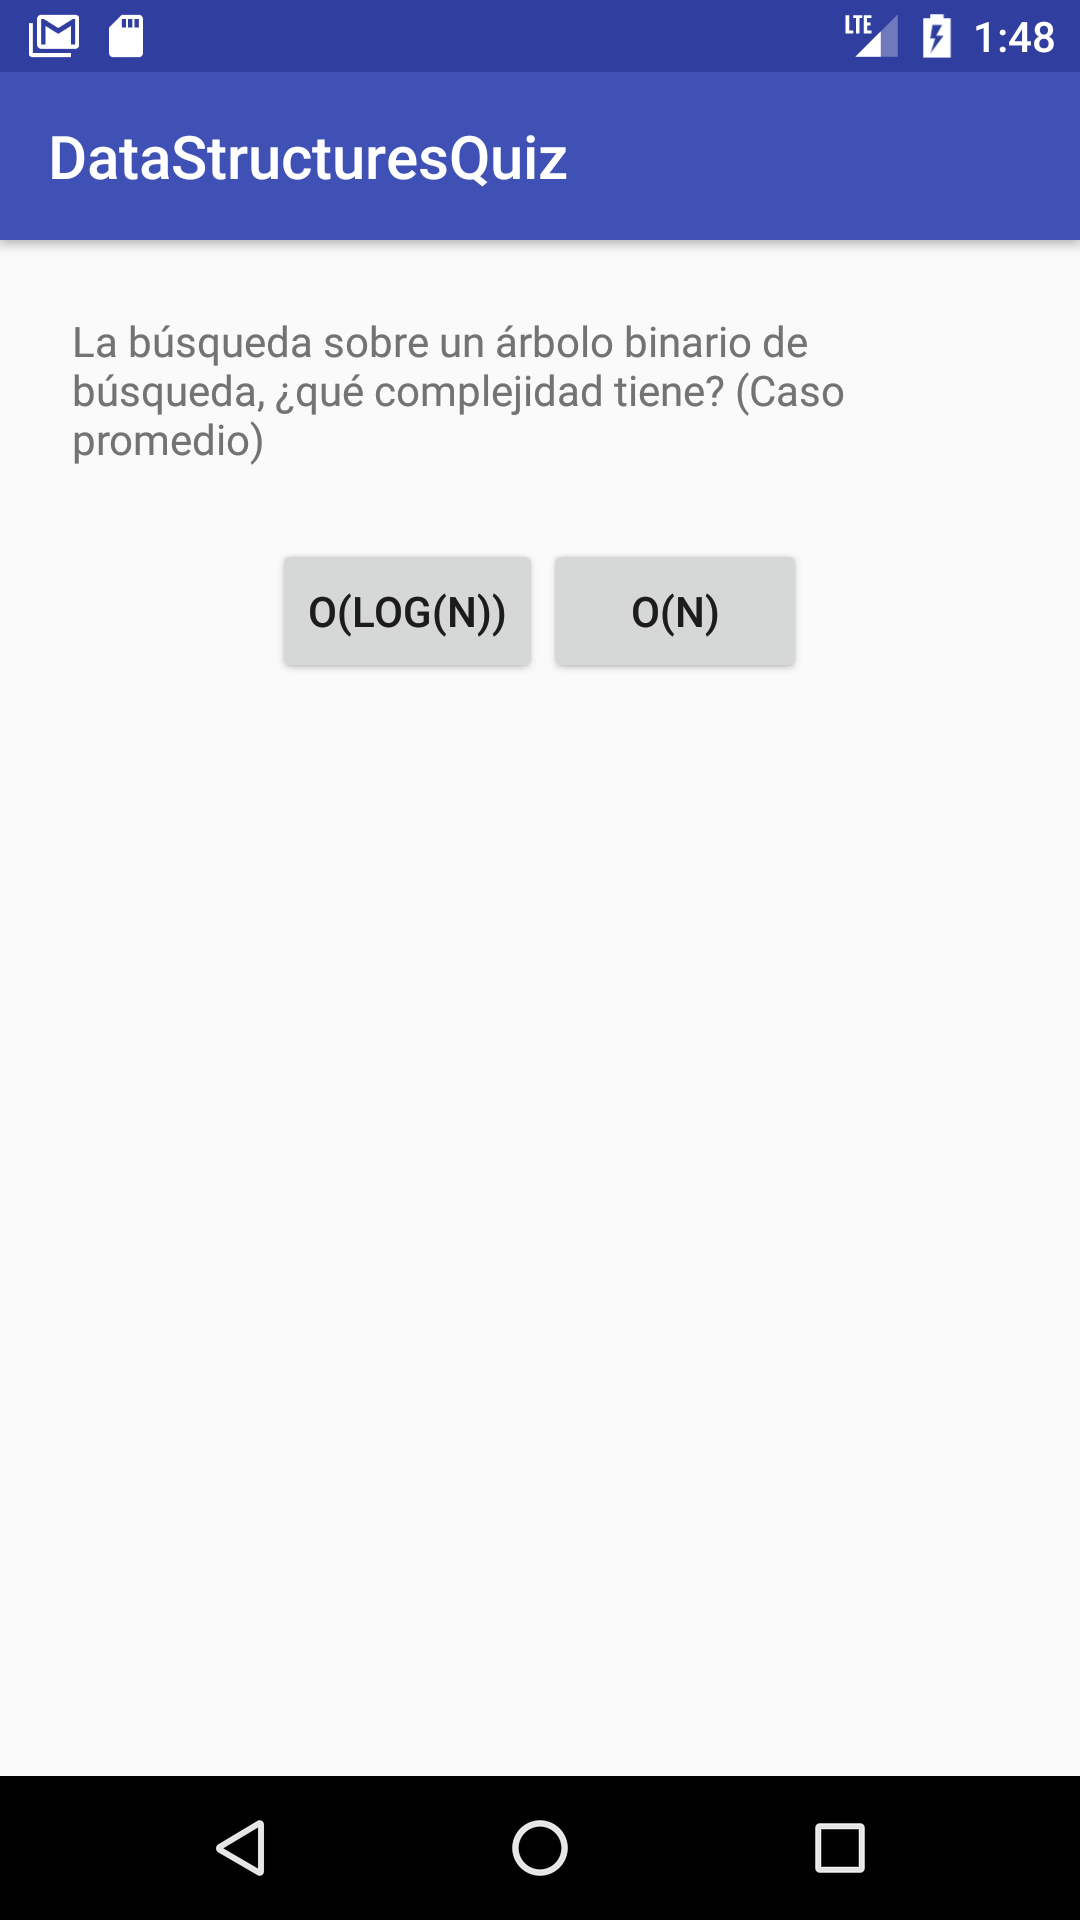
\includegraphics[scale=.1]{quiz_app}}%
    \qquad
    \subfloat[Se muestra el \texttt{Toast} con el mensaje después de dar clic sobre el prime botón]{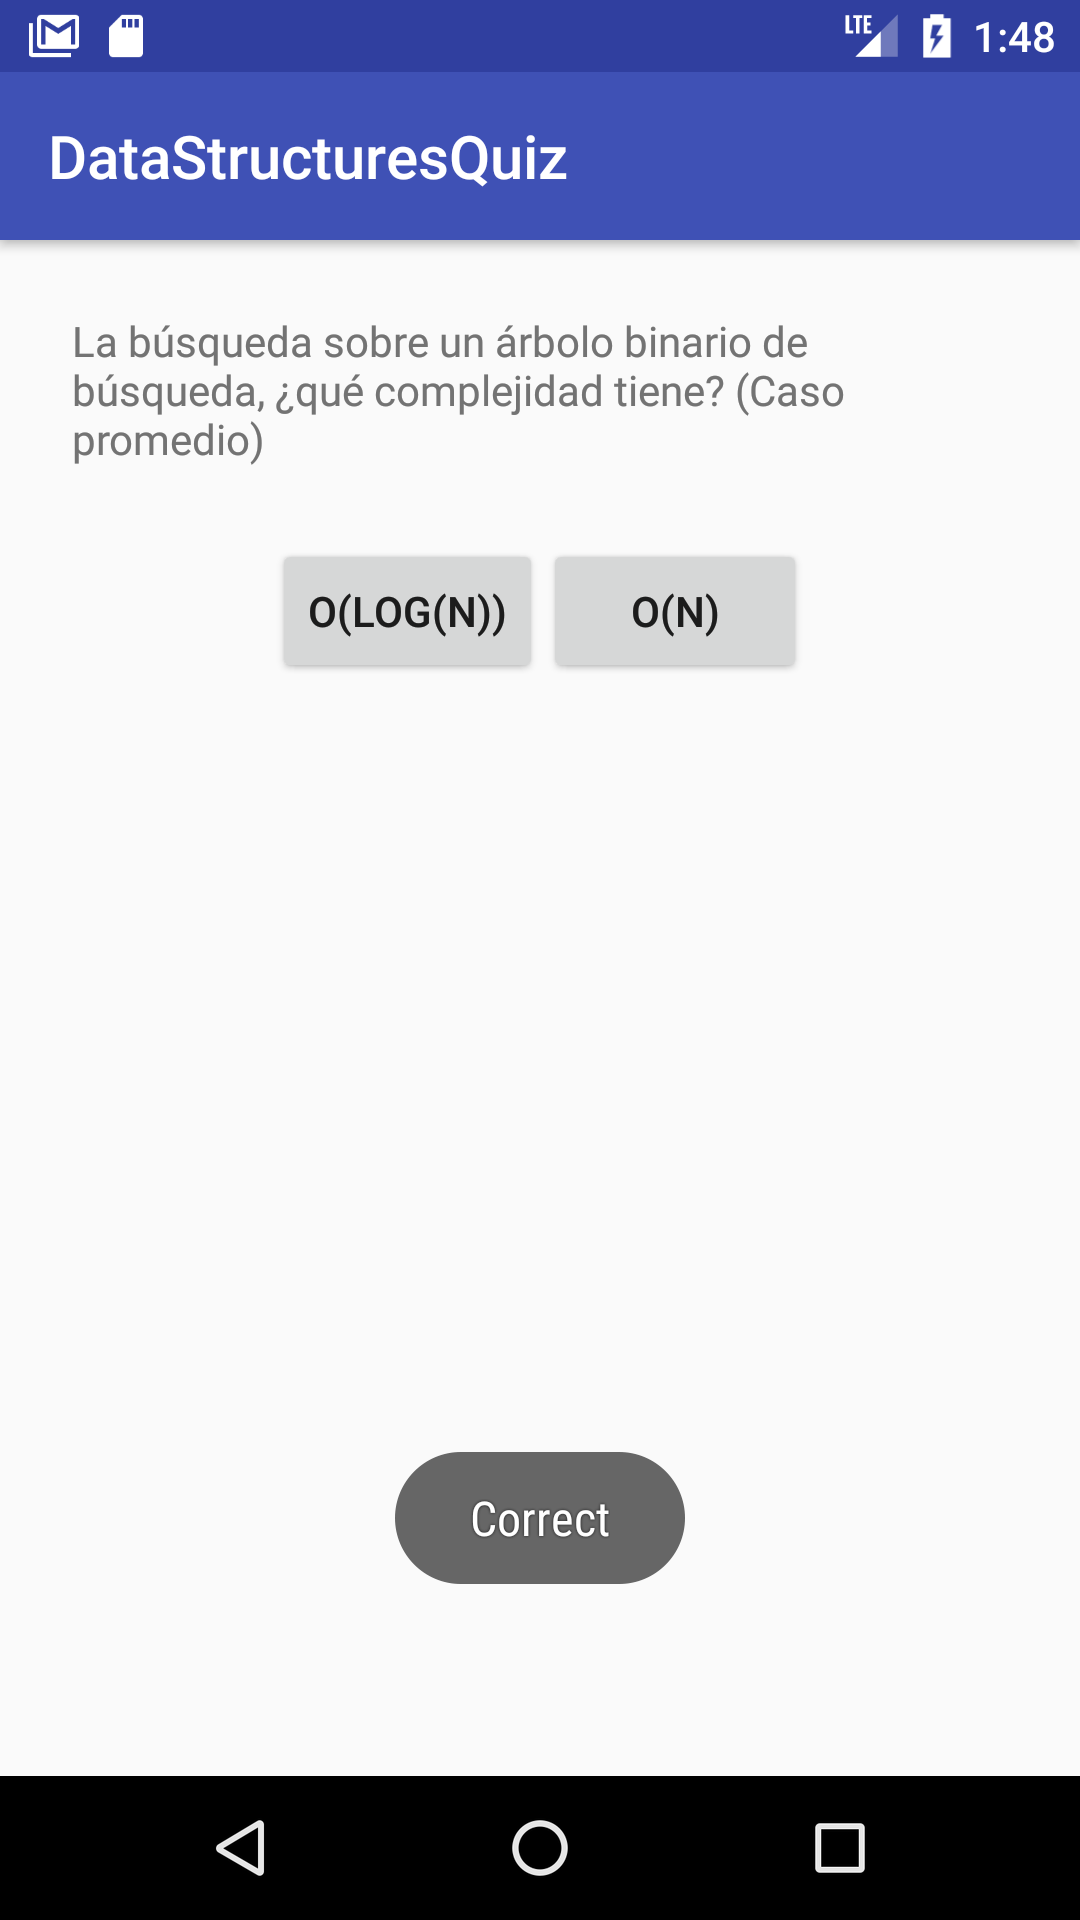
\includegraphics[scale=.1]{quiz_app_clicked} }%
    \caption{Capturas de la ejecución de la aplicación  Data Structures Quiz.}
    \label{fig:quiz_app}%
\end{figure}

\subsection*{SDK para Android de NAOqi}
\label{\detokenize{dev_docs:sdk-para-android-de-naoqi}}
Para ejecutar módulos de manera remota sobre los robots de NAOqi es necesario
contar con un SDK para la plataforma y el lenguaje con el que se desee
desarrollar. La plataforma en cuestión es Android, y Aldebaran brinda un SDK
de Java específicamente para este sistema. Como ya se mencionó en la sección
sobre \sphinxstylestrong{NAOqi}, el SDK de Java utiliza el \sphinxstylestrong{framework qi}.

El SDK provisto  no ha sido actualizado y en el archivo \sphinxstyleemphasis{.jar} no es compatible
con nuevas versiones de Android a partir de la 5.

El SDK se añade al proyecto como si fuera cualquier bibliotecas desarrollada
por un tercero. Cambiando la vista del proyecto que viene por defecto, \sphinxstyleemphasis{Android},
a \sphinxstyleemphasis{Project}, se puede copiar el archivo \sphinxcode{javanaoqi-sdk-2.1.4-android.jar}
al directorio en la ubicación \sphinxstyleemphasis{app/libs}. Después se configura el archivo
del gradle de la aplicación y del proyecto.


\subsubsection{Configuración de Gradle}
\label{\detokenize{dev_docs:configuracion-de-gradle}}
El sistema de construcción de Android Studio está basado en Gradle, y el plugin
de Android para Gradle adiciona varias características que están
construidas específicamente para aplicaciones de Android.\\

\begin{remark}
Gradle es un sistema de automatización de construcción de código abierto
enfocado a la flexibilidad y desempeño.
\end{remark}

La última versión del plugin de Gradle compatible con el SDK que brinda
Aldebaran es la 1.3.1. Por lo tanto después de sumar a nuestro directorio
\sphinxstyleemphasis{app/libs} se configura lo siguiente en el archivo \sphinxcode{buldgradle} del
proyecto:

\fvset{hllines={, ,}}%
\begin{sphinxVerbatim}[commandchars=\\\{\}]
\PYG{n+nx}{buildscript} \PYG{p}{\PYGZob{}}
  \PYG{n+nx}{dependencies} \PYG{p}{\PYGZob{}}
    \PYG{n+nx}{classpath} \PYG{l+s+s1}{\PYGZsq{}com.android.tools.build:gradle:1.3.1\PYGZsq{}}
  \PYG{p}{\PYGZcb{}}
\PYG{p}{\PYGZcb{}}
\end{sphinxVerbatim}

Por último sólo se agrega a las dependencias dentro del archivo \sphinxcode{buildgradle}
de la aplicación \sphinxcode{compilefiles('libs/java-naoqi-sdk-2.1.4-android.jar')}, que
compila el SDK de NAOqi.


\section*{ Firebase para Android}
\label{\detokenize{dev_docs:firebase-para-android}}

% \paragraph{Añadir Firebase a un proyecto de Android}
% \label{\detokenize{dev_docs:anadir-firebase-a-un-proyecto-de-android}}

Los servicios de Firebase utilizados son Firebase Realtime Database
y Authentication. Este último a través de la biblioteca Firebase UI.

Antes de poder utilizar Firebase en una aplicación se debe agregar Firebase a ésta. Después de crear un proyecto en la consola 
de Firebase se siguen los pasos que ésta nos muestra
para añadir Firebase a nuestras aplicaciones ya sea web 
o móviles, en nuestro caso para dispositivos Android.
La consola genera un archivo de configuración
que se añade a la aplicación y luego
se agrega el SDK para poder utilizar las bibliotecas de Firebase en el proyecto.

Cada biblioteca de Firebase que se desee utilizar se añade a las dependencias.
Por ejemplo, sumando a las dependencias de Gradle  \sphinxcode{com.google.firebase:firebase-\\database:11.6.2}
se tiene acceso a a la base de datos en tiempo real que provee Firebase.


\subsection*{Firebase Realtime Database}
\label{\detokenize{dev_docs:firebase-realtime-database}}
Para comenzar a usar la Firebase Realtime Database en la aplicación,
se debe sumar a las dependencias del archivo \sphinxcode{buildgradle}, de la aplicación,
\sphinxcode{'compile.com.google.firebase:firebase-database:11.8.0'}.

%Los datos de Firebase se escriben en una referencia de \sphinxcode{FirebaseDatabase};
%para recuperarlos, se debe adjuntar un agente de escucha o escuchador asíncrono a la
%referencia. El agente de escucha se activa una vez para el estado inicial de los
%datos y otra vez cuando los datos cambian.

%
%\subparagraph{Obtener una DatabaseReference}
%\label{\detokenize{dev_docs:obtener-una-databasereference}}

Para leer y escribir en la base de datos, necesitas una instancia de
\texttt{DatabaseReference}:

\fvset{hllines={, ,}}%
\begin{sphinxVerbatim}[commandchars=\\\{\}]
\PYG{k+kd}{private} \PYG{n}{DatabaseReference} \PYG{n}{mDatabase}\PYG{o}{;}
\PYG{n}{mDatabase} \PYG{o}{=} \PYG{n}{FirebaseDatabase}\PYG{o}{.}\PYG{n+na}{getInstance}\PYG{o}{(}\PYG{o}{)}\PYG{o}{.}\PYG{n+na}{getReference}\PYG{o}{(}\PYG{o}{)}\PYG{o}{;}
\end{sphinxVerbatim}


\subsubsection{Leer y escribir datos}
\label{\detokenize{dev_docs:leer-y-escribir-datos}}
Para ejecutar una escritura básica se usa \sphinxcode{setValue()} para guardar datos en
una referencia que se especifique.

Los tipos de datos que se pueden almacenar son los siguientes:
\begin{itemize}
\item {}
\texttt{String}

\item {}
\texttt{Long}

\item {}
\texttt{Double}

\item {}
\texttt{Boolean}

\item {}
\texttt{Map\textless{}String, Object\textgreater{}}

\item {}
\texttt{List\textless{}Object\textgreater{}}

\end{itemize}

También se puede pasar un objeto personalizado de Java con la restricción
de que la definición de la clase debe tener un constructor predeterminado
que no recibe parámetros y tiene métodos públicos para obtener a los atributos
del objeto.

El siguiente fragmento muestra como escribir un nuevo usuario en la base de
datos.

\fvset{hllines={, ,}}%
\begin{sphinxVerbatim}[commandchars=\\\{\}]
\PYG{k+kd}{public} \PYG{k+kt}{void} \PYG{n+nf}{saveUserToDatabase}\PYG{o}{(}\PYG{n}{String} \PYG{n}{uid}\PYG{o}{,} \PYG{n}{String} \PYG{n}{email}\PYG{o}{)} \PYG{o}{\PYGZob{}}
  \PYG{n}{mDatabase}\PYG{o}{.}\PYG{n+na}{child}\PYG{o}{(}\PYG{l+s}{\PYGZdq{}users/\PYGZdq{}} \PYG{o}{+} \PYG{n}{uid}\PYG{o}{)}\PYG{o}{.}\PYG{n+na}{setValue}\PYG{o}{(}\PYG{n}{email}\PYG{o}{)}\PYG{o}{;}
\PYG{o}{\PYGZcb{}}
\end{sphinxVerbatim}


\subsubsection{Detección de eventos en valores}
\label{\detokenize{dev_docs:detecteccion-eventos-de-valores}}
Para leer datos en una ruta de acceso y escuchar actualizaciones, usa el
método \sphinxcode{addValueEventListener()} o el método \sphinxcode{addListenerForSingleValueEvent()}
para agregar un \sphinxcode{ValueEventListener} a un objetos \sphinxcode{DatabaseReference}.

Un escuchador \sphinxcode{ValueEventListener} de una referencia de la base de datos
tiene una método callback \sphinxcode{onDataChange()} que obtiene una captura estática
del contiene en la ruta determinada.

El ejemplo siguiente es parte de una aplicación que muestra mensajes
almacenados en la base de datos:

\fvset{hllines={, ,}}%
\begin{sphinxVerbatim}[commandchars=\\\{\}]
\PYG{n}{mMessagesReference}\PYG{o}{.}\PYG{n+na}{addValueEventListener}\PYG{o}{(}\PYG{k}{new} \PYG{n}{ValueEventListener}\PYG{o}{(}\PYG{o}{)}\PYG{o}{\PYGZob{}}
  \PYG{n+nd}{@Override}
  \PYG{k+kd}{public} \PYG{k+kt}{void} \PYG{n+nf}{onDataChange}\PYG{o}{(}\PYG{n}{DataSnapshot} \PYG{n}{snapshot}\PYG{o}{)} \PYG{o}{\PYGZob{}}
    \PYG{n}{Message} \PYG{n}{msg} \PYG{o}{=} \PYG{n}{snapshot}\PYG{o}{.}\PYG{n+na}{getValue}\PYG{o}{(}\PYG{n}{Message}\PYG{o}{.}\PYG{n+na}{class}\PYG{o}{)}\PYG{o}{;}
    \PYG{c+c1}{//...}
  \PYG{o}{\PYGZcb{}}
\PYG{o}{\PYGZcb{}}\PYG{o}{)}
\end{sphinxVerbatim}

El escuchador recibe un objeto \sphinxcode{DataSnapshot} que contiene los datos de la
ubicación especifica al momentos del evento.

La diferencia entre \sphinxcode{addValueEventListener()} y
\sphinxcode{addListenerForSingleValue\\Event()} es que el primero se suscribe a cierta
ubicación para escuchar cambios, y el segundo lee los datos de una ubicación
una sola vez.


\subsubsection{Actualización o borrado de datos}
\label{\detokenize{dev_docs:actulizacion-o-borrado-de-datos}}
Para actualizar se llama al método \sphinxcode{update\\Children()} y para eliminar datos
en una referencia se usa \sphinxcode{removeValue} o se pasa como parámetro un valor
\sphinxcode{null} a \sphinxcode{setValue()}.

También existe el método \sphinxcode{push()} para añadir una entrada con un identificador
único sobre una referencia.


\subsection*{Firebase UI Authentication}
\label{\detokenize{dev_docs:firebase-ui-authentication}}
%FirebaseUI es una biblioteca de código abierto que ofrece referencias a la IU
%de manera simple y personalizable, sobre los SDK de Firebase, para eliminar
%código repetitivo y promover mejores prácticas (en cuanto a la experiencia
%de usuario y seguridad) para la autenticación.

Es una API para manejar el flujo del inicio de sesión con una
dirección de correo electrónico, números de teléfono, y a través de
proveedores como Google Sign-In, y Facebook Login. Está construido sobre
Firebase Authentication.

%FirebaseUI se integra con \sphinxstylestrong{Smart Lock} para guardar y recuperar credenciales,
%habilita el inicio de sesión con un solo click en una aplicación cuando el
%usuario regresa a esta. Maneja casos de uso complicados como la recuperación
%de la cuenta y el enlace con la cuenta que son inseguros y difíciles de implementar
%usando la API base de Firebase Authentication.


\subsubsection{Configuración}
\label{\detokenize{dev_docs:configuracion}}
Como prerrequisito, la aplicación debe estar configurada para utilizar Firebase.
Después, se agrega a la biblioteca de FirebaseUI auth en las dependencias de
\sphinxcode{buildgradle} de la aplicación.

\fvset{hllines={, ,}}%
\begin{sphinxVerbatim}[commandchars=\\\{\}]
\PYG{n+nx}{dependencies} \PYG{p}{\PYGZob{}}
  \PYG{n+nx}{compile} \PYG{l+s+s1}{\PYGZsq{}com.firebaseui:firebase\PYGZhy{}ui\PYGZhy{}auth:3.0.0\PYGZsq{}}
\PYG{p}{\PYGZcb{}}
\end{sphinxVerbatim}


\subsubsection{Uso de FirebaseUI para autenticación}
\label{\detokenize{dev_docs:uso-de-firebaseui-para-autenticacion}}
Antes de llamar al flujo de autenticación de FirebaseUI, la aplicación debe
checar que un usuario ya esté registrado de una sesión previa. Este caso
es cuando el usuario inicio sesión y salió de la aplicación para luego regresar
a esta.

\fvset{hllines={, ,}}%
\begin{sphinxVerbatim}[commandchars=\\\{\}]
\PYG{n}{FirebaseAuth} \PYG{n}{auth} \PYG{o}{=} \PYG{n}{FirebaseAuth}\PYG{o}{.}\PYG{n+na}{getInstance}\PYG{o}{(}\PYG{o}{)}\PYG{o}{;}
\PYG{k}{if} \PYG{o}{(}\PYG{n}{auth}\PYG{o}{.}\PYG{n+na}{getCurrentUser}\PYG{o}{(}\PYG{o}{)} \PYG{o}{!}\PYG{o}{=} \PYG{k+kc}{null}\PYG{o}{)} \PYG{o}{\PYGZob{}}
  \PYG{c+c1}{// el usuario tiene abierta la sesión}
\PYG{o}{\PYGZcb{}} \PYG{k}{else} \PYG{o}{\PYGZob{}}
  \PYG{c+c1}{// el usuario no ha iniciado sesión}
\PYG{o}{\PYGZcb{}}
\end{sphinxVerbatim}

El punto de entrada para el flujo de la autenticación es la clase
\sphinxcode{com.firebase.ui.auth.AuthUI}.


\subsubsection{Inicio de sesión}
\label{\detokenize{dev_docs:inicio-de-sesion}}
Si un usuario no ha iniciado sesión, entonces el proceso de inicio de sesión
puede empezar creando un intent sign-in usando \sphinxcode{AuthUISignInIntent\\Builder}.
Se puede recuperar una instancia del constructor llamando
\sphinxcode{createSignIn\\IntentBuilder()} en la instancia retomada de AuthUI.

El constructor provee las siguientes opciones de personalización para el flujo
de la autenticación:
\begin{itemize}
\item {} 
El conjunto de proveedores de autenticación puede especificarse (Google, Twitter, Facebook)

\item {} 
Un URL con los términos de servicio para la aplicación.

\item {} 
Un tema personalizado puede ser especificado para el flujo, el cual se aplica a todas las actividades en el flujo para que haya consistencia de colores y tipografía.

\end{itemize}

Si no se requiere personalizar , y solo se necesita el correo electrónico para
autenticarse, el flujo del inicio de sesión comienza como sigue:

\fvset{hllines={, ,}}%
\begin{sphinxVerbatim}[commandchars=\\\{\}]
\PYG{c+c1}{// Un valor para el código de petición arbitrario}
\PYG{k+kd}{private} \PYG{k+kd}{static} \PYG{k+kd}{final} \PYG{k+kt}{int} \PYG{n}{RC\PYGZus{}SIGN\PYGZus{}IN} \PYG{o}{=} \PYG{l+m+mi}{123}\PYG{o}{;}

\PYG{c+c1}{// ...}

\PYG{n}{startActivityForResult}\PYG{o}{(}
  \PYG{c+c1}{// obtiene una instancia de AuthUI basado en la aplicación por defecto}
  \PYG{n}{AuthUI}\PYG{o}{.}\PYG{n+na}{getInstance}\PYG{o}{(}\PYG{o}{)}\PYG{o}{.}\PYG{n+na}{createSignInIntentBuilder}\PYG{o}{(}\PYG{o}{)}\PYG{o}{.}\PYG{n+na}{build}\PYG{o}{(}\PYG{o}{)}\PYG{o}{,}
  \PYG{n}{RC\PYGZus{}SIGN\PYGZus{}IN}\PYG{o}{)}\PYG{o}{;}
\end{sphinxVerbatim}

El segundo parámetro de \sphinxcode{startActivityForResult()} (\sphinxcode{RC\_SIGN\_IN})  es un
código de petición para identificar la petición cuando el resultado retorna
a la aplicación en el métodos \sphinxcode{onActivityResult()}.

El flujo de la autenticación suministra varios códigos de respuesta, entre
los más comunes están:
\begin{itemize}
\item {} 
\sphinxcode{Activity.RESULT\_OK}, si es el usuario inició sesión.

\item {} 
\sphinxcode{Activity.RESULT\_CANCELLED}, si el usuario canceló manualmente el inicio de sesión.

\item {} 
\sphinxcode{ErrorCodes.NO\_NETWORK}, si no hay conexión a una red.

\item {} 
\sphinxcode{ErrorCodes.UNKNOWN\_ERROR},  todos los otros errores.

\end{itemize}

Siguiendo con el ejemplo del inicio de sesión con el correo electrónico,
el método \sphinxcode{onActivityResult()} queda como sigue:

\fvset{hllines={, ,}}%
\begin{sphinxVerbatim}[commandchars=\\\{\}]
\PYG{k+kd}{protected} \PYG{k+kt}{void} \PYG{n+nf}{onActivityResult}\PYG{o}{(}\PYG{k+kt}{int} \PYG{n}{requestCode}\PYG{o}{,} \PYG{k+kt}{int} \PYG{n}{resultCode}\PYG{o}{,} \PYG{n}{Intent} \PYG{n}{data}\PYG{o}{)} \PYG{o}{\PYGZob{}}
    \PYG{k+kd}{super}\PYG{o}{.}\PYG{n+na}{onActivityResult}\PYG{o}{(}\PYG{n}{requestCode}\PYG{o}{,} \PYG{n}{resultCode}\PYG{o}{,} \PYG{n}{data}\PYG{o}{)}\PYG{o}{;}
    \PYG{c+c1}{// RC\PYGZus{}SIGN\PYGZus{}IN es el segundo parámetro que se pasó a startActivityForResult}
    \PYG{k}{if} \PYG{o}{(}\PYG{n}{requestCode} \PYG{o}{=}\PYG{o}{=} \PYG{n}{RC\PYGZus{}SIGN\PYGZus{}IN}\PYG{o}{)} \PYG{o}{\PYGZob{}}
        \PYG{n}{IdpResponse} \PYG{n}{response} \PYG{o}{=} \PYG{n}{IdpResponse}\PYG{o}{.}\PYG{n+na}{fromResultIntent}\PYG{o}{(}\PYG{n}{data}\PYG{o}{)}\PYG{o}{;}

        \PYG{c+c1}{// Si el usuario inició sesión exitosamente}
        \PYG{k}{if} \PYG{o}{(}\PYG{n}{resultCode} \PYG{o}{=}\PYG{o}{=} \PYG{n}{RESULT\PYGZus{}OK}\PYG{o}{)} \PYG{o}{\PYGZob{}}
            \PYG{n}{startActivity}\PYG{o}{(}\PYG{n}{SignedInActivity}\PYG{o}{.}\PYG{n+na}{createIntent}\PYG{o}{(}\PYG{k}{this}\PYG{o}{,} \PYG{n}{response}\PYG{o}{)}\PYG{o}{)}\PYG{o}{;}
            \PYG{n}{finish}\PYG{o}{(}\PYG{o}{)}\PYG{o}{;}
        \PYG{o}{\PYGZcb{}} \PYG{k}{else} \PYG{o}{\PYGZob{}}
            \PYG{c+c1}{// El inicio de sesión falló}
            \PYG{k}{if} \PYG{o}{(}\PYG{n}{response} \PYG{o}{=}\PYG{o}{=} \PYG{k+kc}{null}\PYG{o}{)} \PYG{o}{\PYGZob{}}
                \PYG{c+c1}{// El usuario presión el botón de regresar}
                \PYG{n}{showSnackbar}\PYG{o}{(}\PYG{n}{R}\PYG{o}{.}\PYG{n+na}{string}\PYG{o}{.}\PYG{n+na}{sign\PYGZus{}in\PYGZus{}cancelled}\PYG{o}{)}\PYG{o}{;}
                \PYG{k}{return}\PYG{o}{;}
            \PYG{o}{\PYGZcb{}}

            \PYG{k}{if} \PYG{o}{(}\PYG{n}{response}\PYG{o}{.}\PYG{n+na}{getError}\PYG{o}{(}\PYG{o}{)}\PYG{o}{.}\PYG{n+na}{getErrorCode}\PYG{o}{(}\PYG{o}{)} \PYG{o}{=}\PYG{o}{=} \PYG{n}{ErrorCodes}\PYG{o}{.}\PYG{n+na}{NO\PYGZus{}NETWORK}\PYG{o}{)} \PYG{o}{\PYGZob{}}
                \PYG{n}{showSnackbar}\PYG{o}{(}\PYG{n}{R}\PYG{o}{.}\PYG{n+na}{string}\PYG{o}{.}\PYG{n+na}{no\PYGZus{}internet\PYGZus{}connection}\PYG{o}{)}\PYG{o}{;}
                \PYG{k}{return}\PYG{o}{;}
            \PYG{o}{\PYGZcb{}}
            \PYG{n}{showSnackbar}\PYG{o}{(}\PYG{n}{R}\PYG{o}{.}\PYG{n+na}{string}\PYG{o}{.}\PYG{n+na}{unknown\PYGZus{}error}\PYG{o}{)}\PYG{o}{;}
            \PYG{n}{Log}\PYG{o}{.}\PYG{n+na}{e}\PYG{o}{(}\PYG{n}{TAG}\PYG{o}{,} \PYG{l+s}{\PYGZdq{}Sign\PYGZhy{}in error: \PYGZdq{}}\PYG{o}{,} \PYG{n}{response}\PYG{o}{.}\PYG{n+na}{getError}\PYG{o}{(}\PYG{o}{)}\PYG{o}{)}\PYG{o}{;}
        \PYG{o}{\PYGZcb{}}
    \PYG{o}{\PYGZcb{}}
\PYG{o}{\PYGZcb{}}
\end{sphinxVerbatim}


\subsubsection{Cierre de sesión}
\label{\detokenize{dev_docs:cierre-de-sesion}}
AuthUI brinda un método \sphinxcode{signOut} simple que encapsula todo el proceso
que conlleva un cierre de sesión. El método retornar una objeto \sphinxcode{Task}
que se marca completamente una vez que todo el proceso de cierre de sesión
se ha completado.

\fvset{hllines={, ,}}%
\begin{sphinxVerbatim}[commandchars=\\\{\}]
\PYG{k+kd}{public} \PYG{k+kt}{void} \PYG{n+nf}{signOut}\PYG{o}{(}\PYG{o}{)}\PYG{o}{\PYGZob{}}
    \PYG{n}{AuthUI}\PYG{o}{.}\PYG{n+na}{getInstance}\PYG{o}{(}\PYG{o}{)}\PYG{o}{.}\PYG{n+na}{signOut}\PYG{o}{(}\PYG{k}{this}\PYG{o}{)}
            \PYG{o}{.}\PYG{n+na}{addOnCompleteListener}\PYG{o}{(}\PYG{k}{new} \PYG{n}{OnCompleteListener}\PYG{o}{\PYGZlt{}}\PYG{n}{Void}\PYG{o}{\PYGZgt{}}\PYG{o}{(}\PYG{o}{)} \PYG{o}{\PYGZob{}}
                \PYG{n+nd}{@Override}
                \PYG{k+kd}{public} \PYG{k+kt}{void} \PYG{n+nf}{onComplete}\PYG{o}{(}\PYG{n+nd}{@NonNull} \PYG{n}{Task}\PYG{o}{\PYGZlt{}}\PYG{n}{Void}\PYG{o}{\PYGZgt{}} \PYG{n}{task}\PYG{o}{)} \PYG{o}{\PYGZob{}}
                    \PYG{k}{if} \PYG{o}{(}\PYG{n}{task}\PYG{o}{.}\PYG{n+na}{isSuccessful}\PYG{o}{(}\PYG{o}{)}\PYG{o}{)} \PYG{o}{\PYGZob{}}
                        \PYG{n}{startActivity}\PYG{o}{(}\PYG{n}{MyActivity}\PYG{o}{.}\PYG{n+na}{createIntent}\PYG{o}{(}\PYG{n}{SignInActivity}\PYG{o}{.}\PYG{n+na}{this}\PYG{o}{)}\PYG{o}{)}\PYG{o}{;}
                        \PYG{n}{finish}\PYG{o}{(}\PYG{o}{)}\PYG{o}{;}
                    \PYG{o}{\PYGZcb{}} \PYG{k}{else} \PYG{o}{\PYGZob{}}
                        \PYG{c+c1}{// Falló el cierre de sesión}
                    \PYG{o}{\PYGZcb{}}
                \PYG{o}{\PYGZcb{}}
            \PYG{o}{\PYGZcb{}}\PYG{o}{)}\PYG{o}{;}
\PYG{o}{\PYGZcb{}}
\end{sphinxVerbatim}


\section*{ ButterKnife}
\label{\detokenize{dev_docs:butterknife}}
ButterKnife es una biblioteca de viewbinding, esto quiere decir que genera
objetos view a partir de recursos, pero lo que la hace especial es que evita
el código repetitivo, como llamar a la función \sphinxcode{findViewById}. ButterKnife
ayuda a enlazar atributos, métodos y views.


\subsection*{Configuración}
\label{\detokenize{dev_docs:id1}}
Para comenzar a utilizar butterknife en un proyecto. Solo se agrega a Las
dependencias del \sphinxcode{buildgradle} lo siguiente:

\fvset{hllines={, ,}}%
\begin{sphinxVerbatim}[commandchars=\\\{\}]
\PYG{n+nx}{compile} \PYG{l+s+s1}{\PYGZsq{}com.jakewharton:butterknife:8.8.1\PYGZsq{}}
\PYG{n+nx}{provided} \PYG{l+s+s1}{\PYGZsq{}com.jakewharton:butterknife\PYGZhy{}compiler:8.8.1\PYGZsq{}}
\end{sphinxVerbatim}


\subsection*{Uso}
\label{\detokenize{dev_docs:uso}}
Para entender mejor las características que tiene ButterKnife supongamos que
tenemos una actividad con un botón que reaccione a clics. Sin usar ButterKnife
la actividad queda como sigue:

\fvset{hllines={, ,}}%
\begin{sphinxVerbatim}[commandchars=\\\{\}]
\PYG{k+kd}{public} \PYG{k+kd}{class} \PYG{n+nc}{MainActivity} \PYG{k+kd}{extends} \PYG{n}{AppCompatActivity} \PYG{o}{\PYGZob{}}
  \PYG{k+kd}{private} \PYG{n}{TextView} \PYG{n}{mTextView}\PYG{o}{;}
  \PYG{k+kd}{private} \PYG{n}{Button} \PYG{n}{mButton}\PYG{o}{;}

  \PYG{n+nd}{@Override}
  \PYG{k+kd}{protected} \PYG{k+kt}{void} \PYG{n+nf}{onCreate}\PYG{o}{(}\PYG{n}{Bundle} \PYG{n}{savedInstanceState}\PYG{o}{)} \PYG{o}{\PYGZob{}}
      \PYG{k+kd}{super}\PYG{o}{.}\PYG{n+na}{onCreate}\PYG{o}{(}\PYG{n}{savedInstanceState}\PYG{o}{)}\PYG{o}{;}
      \PYG{n}{setContentView}\PYG{o}{(}\PYG{n}{R}\PYG{o}{.}\PYG{n+na}{layout}\PYG{o}{.}\PYG{n+na}{activity\PYGZus{}main}\PYG{o}{)}\PYG{o}{;}

      \PYG{n}{mButton} \PYG{o}{=} \PYG{o}{(}\PYG{n}{Button}\PYG{o}{)} \PYG{n}{findViewById}\PYG{o}{(}\PYG{n}{R}\PYG{o}{.}\PYG{n+na}{id}\PYG{o}{.}\PYG{n+na}{AButton}\PYG{o}{)}\PYG{o}{;}
      \PYG{n}{mTextView} \PYG{o}{=} \PYG{o}{(}\PYG{n}{TextView}\PYG{o}{)} \PYG{n}{findViewById}\PYG{o}{(}\PYG{n}{R}\PYG{o}{.}\PYG{n+na}{id}\PYG{o}{.}\PYG{n+na}{texView}\PYG{o}{)}\PYG{o}{;}

      \PYG{n}{mAOptionButton}\PYG{o}{.}\PYG{n+na}{setOnClickListener}\PYG{o}{(}\PYG{k}{new} \PYG{n}{View}\PYG{o}{.}\PYG{n+na}{OnClickListener}\PYG{o}{(}\PYG{o}{)} \PYG{o}{\PYGZob{}}
          \PYG{n+nd}{@Override}
          \PYG{k+kd}{public} \PYG{k+kt}{void} \PYG{n+nf}{onClick}\PYG{o}{(}\PYG{n}{View} \PYG{n}{view}\PYG{o}{)} \PYG{o}{\PYGZob{}}
           \PYG{c+c1}{// Haz algo}
          \PYG{o}{\PYGZcb{}}
      \PYG{o}{\PYGZcb{}}\PYG{o}{)}\PYG{o}{;}
    \PYG{o}{\PYGZcb{}}
  \PYG{o}{\PYGZcb{}}
\end{sphinxVerbatim}

Utilizando ButterKnife la actividad cambiaría a los siguiente:

\fvset{hllines={, ,}}%
\begin{sphinxVerbatim}[commandchars=\\\{\}]
\PYG{k+kd}{public} \PYG{k+kd}{class} \PYG{n+nc}{MainActivity} \PYG{k+kd}{extends} \PYG{n}{AppCompatActivity} \PYG{o}{\PYGZob{}}
  \PYG{n+nd}{@BindView}\PYG{o}{(}\PYG{n}{R}\PYG{o}{.}\PYG{n+na}{id}\PYG{o}{.}\PYG{n+na}{textView}\PYG{o}{)}
  \PYG{n}{TextView} \PYG{n}{mTextView}\PYG{o}{;}

  \PYG{n+nd}{@Override}
  \PYG{k+kd}{protected} \PYG{k+kt}{void} \PYG{n+nf}{onCreate}\PYG{o}{(}\PYG{n}{Bundle} \PYG{n}{savedInstanceState}\PYG{o}{)} \PYG{o}{\PYGZob{}}
      \PYG{k+kd}{super}\PYG{o}{.}\PYG{n+na}{onCreate}\PYG{o}{(}\PYG{n}{savedInstanceState}\PYG{o}{)}\PYG{o}{;}
      \PYG{n}{setContentView}\PYG{o}{(}\PYG{n}{R}\PYG{o}{.}\PYG{n+na}{layout}\PYG{o}{.}\PYG{n+na}{activity\PYGZus{}main}\PYG{o}{)}\PYG{o}{;}
      \PYG{c+c1}{// Enlaza butterknife a la actividad}
      \PYG{n}{ButterKnife}\PYG{o}{.}\PYG{n+na}{bind}\PYG{o}{(}\PYG{k}{this}\PYG{o}{)}\PYG{o}{;}
  \PYG{o}{\PYGZcb{}}

  \PYG{n+nd}{@OnClick}\PYG{o}{(}\PYG{n}{R}\PYG{o}{.}\PYG{n+na}{id}\PYG{o}{.}\PYG{n+na}{AButton}\PYG{o}{)}
  \PYG{k+kd}{public} \PYG{k+kt}{void} \PYG{n+nf}{OnClickMyButton}\PYG{o}{(}\PYG{o}{)} \PYG{o}{\PYGZob{}}
    \PYG{c+c1}{// Haz algo}
  \PYG{o}{\PYGZcb{}}

\PYG{o}{\PYGZcb{}}
\end{sphinxVerbatim}

Al comparar se nota como evita duplicar código, y el código de los escuchadores
es mucho más simple y parece explicarse por sí mismo.


\section*{ Volley}
\label{\detokenize{dev_docs:volley}}
Volley es una biblioteca HTTP que facilita el acceso a la red en aplicaciones
de Android. Algunos de sus beneficios son los siguientes:
\begin{itemize}
\item {} 
Programación automática de peticiones a través de la red.

\item {} 
Múltiples conexiones concurrentes.

\item {} 
Soporte para priorizar peticiones.

\item {} 
Una API para cancelar peticiones.

\item {} 
Personalizable, por ejemplo, se puede añadir la opción de reintentar un petición.

\end{itemize}


\subsection*{Configuración}
\label{\detokenize{dev_docs:id2}}
La manera más sencilla de añadir Volley a un proyecto es a través de la dependencia
en el \sphinxcode{buildgradle} de la aplicación.

\fvset{hllines={, ,}}%
\begin{sphinxVerbatim}[commandchars=\\\{\}]
\PYG{n+nx}{dependencies} \PYG{p}{\PYGZob{}}
\PYG{p}{...}
\PYG{n+nx}{compile} \PYG{l+s+s1}{\PYGZsq{}com.android.volley:volley:1.1.0\PYGZsq{}}
\PYG{p}{\PYGZcb{}}
\end{sphinxVerbatim}


\subsection*{Enviando una petición simple}
\label{\detokenize{dev_docs:enviando-una-peticion-simple}}
A un alto nivel, se utiliza Volley creando un objeto \sphinxcode{RequestQueue} y
pasándole objetos \sphinxcode{Request}. \sphinxcode{RequestQueue} administra hilos trabajadores
para ejecutar operaciones en red, leyendo y escribiendo desde el caché, y
parseando respuestas. Las peticiones hacen el parseo de respuestas en crudo
y Volley se ocupa de remitir la respuesta parseada de regreso al hilo principal
para su entrega.

Volley provee una método \sphinxcode{VolleynewRequestQueue} que prepara una
\sphinxcode{RequestQueue}, usando valores por defecto, e inicia la cola. El
siguiente ejemplo presenta cómo se crea una nueva cola de peticiones,
así como una simple petición \sphinxcode{GET} a \sphinxcode{www.google.com}, recibiendo  la respuesta
en una cadena y mostrándola en un \sphinxcode{TextView}.

\fvset{hllines={, ,}}%
\begin{sphinxVerbatim}[commandchars=\\\{\}]
\PYG{n+nd}{@BindView}\PYG{o}{(}\PYG{n}{R}\PYG{o}{.}\PYG{n+na}{id}\PYG{o}{.}\PYG{n+na}{text}\PYG{o}{)}
\PYG{n}{TextView} \PYG{n}{mTextView}\PYG{o}{;}

\PYG{c+c1}{// Instancia a la cola de peticiones}
\PYG{n}{RequestQueue} \PYG{n}{queue} \PYG{o}{=} \PYG{n}{Volley}\PYG{o}{.}\PYG{n+na}{newRequestQueue}\PYG{o}{(}\PYG{k}{this}\PYG{o}{)}\PYG{o}{;}
\PYG{n}{String} \PYG{n}{url} \PYG{o}{=}\PYG{l+s}{\PYGZdq{}http://www.google.com\PYGZdq{}}\PYG{o}{;}

\PYG{c+c1}{// Solicita una respuesta en formato de cadena haciendo un GET al URL}
\PYG{n}{StringRequest} \PYG{n}{stringRequest} \PYG{o}{=} \PYG{k}{new} \PYG{n}{StringRequest}\PYG{o}{(}\PYG{n}{Request}\PYG{o}{.}\PYG{n+na}{Method}\PYG{o}{.}\PYG{n+na}{GET}\PYG{o}{,} \PYG{n}{url}\PYG{o}{,}
          \PYG{k}{new} \PYG{n}{Response}\PYG{o}{.}\PYG{n+na}{Listener}\PYG{o}{\PYGZlt{}}\PYG{n}{String}\PYG{o}{\PYGZgt{}}\PYG{o}{(}\PYG{o}{)} \PYG{o}{\PYGZob{}}
  \PYG{n+nd}{@Override}
  \PYG{k+kd}{public} \PYG{k+kt}{void} \PYG{n+nf}{onResponse}\PYG{o}{(}\PYG{n}{String} \PYG{n}{response}\PYG{o}{)} \PYG{o}{\PYGZob{}}
      \PYG{n}{mTextView}\PYG{o}{.}\PYG{n+na}{setText}\PYG{o}{(}\PYG{l+s}{\PYGZdq{}Response is: \PYGZdq{}}\PYG{o}{+} \PYG{n}{response}\PYG{o}{.}\PYG{n+na}{substring}\PYG{o}{(}\PYG{l+m+mi}{0}\PYG{o}{,}\PYG{l+m+mi}{500}\PYG{o}{)}\PYG{o}{)}\PYG{o}{;}
  \PYG{o}{\PYGZcb{}}
\PYG{o}{\PYGZcb{}}\PYG{o}{,} \PYG{k}{new} \PYG{n}{Response}\PYG{o}{.}\PYG{n+na}{ErrorListener}\PYG{o}{(}\PYG{o}{)} \PYG{o}{\PYGZob{}}
  \PYG{n+nd}{@Override}
  \PYG{k+kd}{public} \PYG{k+kt}{void} \PYG{n+nf}{onErrorResponse}\PYG{o}{(}\PYG{n}{VolleyError} \PYG{n}{error}\PYG{o}{)} \PYG{o}{\PYGZob{}}
      \PYG{n}{mTextView}\PYG{o}{.}\PYG{n+na}{setText}\PYG{o}{(}\PYG{l+s}{\PYGZdq{}That didn\PYGZsq{}t work!\PYGZdq{}}\PYG{o}{)}\PYG{o}{;}
  \PYG{o}{\PYGZcb{}}
\PYG{o}{\PYGZcb{}}\PYG{o}{)}\PYG{o}{;}
\PYG{c+c1}{// Añade la petición a la cola RequestQueue}
\PYG{n}{queue}\PYG{o}{.}\PYG{n+na}{add}\PYG{o}{(}\PYG{n}{stringRequest}\PYG{o}{)}\PYG{o}{;}
\end{sphinxVerbatim}

Volley siempre entrega respuestas parseadas sobre el hilo principal. Ejecutarlo
sobre el hilo principal es conveniente para poblar elementos de la interfaz de
usuario con los datos recibidos.